\documentclass[10pt,letterpaper]{article}
\usepackage[margin=0.82in]{geometry}
\usepackage[T1]{fontenc}
\usepackage{lmodern,microtype}
\usepackage{amsmath,amssymb,booktabs,tabularx,array}
\usepackage{xcolor,tikz}
\usetikzlibrary{arrows.meta,positioning}
\usepackage{enumitem}
\usepackage{hyperref}
\usepackage{fancyhdr}
\definecolor{ink}{HTML}{16334A}
\definecolor{accent}{HTML}{087F8C}
\definecolor{wash}{HTML}{EDF5F6}
\hypersetup{colorlinks=true,linkcolor=ink,urlcolor=accent,citecolor=accent,
  pdftitle={From a Fresh Save to First Bowser: GPT-6 Astra and Code as Policy in Super Mario 64},
  pdfauthor={SM64 Policy Lab; development agent: GPT-6 Astra}}
\pagestyle{fancy}\fancyhf{}
\fancyhead[L]{\small\textcolor{ink}{SM64 Policy Lab}}
\fancyhead[R]{\small Technical report / September 2026}
\fancyfoot[C]{\thepage}
\setlength{\headheight}{14pt}
\setlength{\parindent}{0pt}\setlength{\parskip}{5pt}
\setlist[itemize]{nosep,leftmargin=1.3em}
\setlist[enumerate]{nosep,leftmargin=1.5em}
\newcolumntype{Y}{>{\raggedright\arraybackslash}X}
\newcommand{\code}[1]{\texttt{#1}}
\newcommand{\clip}{\operatorname{clip}}
\newcommand{\wrap}{\operatorname{wrap}}
\newcommand{\popcount}{\operatorname{popcount}}
\begin{document}
\thispagestyle{empty}
{\small\textcolor{accent}{TECHNICAL REPORT \quad / \quad SEPTEMBER 28, 2026}}
\vspace{0.3cm}

{\LARGE\bfseries\color{ink} From a Fresh Save to First Bowser:\\[3pt]
GPT-6 Astra and Code as Policy\\[3pt] in Super Mario 64\par}
\vspace{0.2cm}
{\large Development agent: \textbf{GPT-6 Astra}}\\
Human-directed experiment in SM64 Policy Lab

\begin{abstract}
\noindent We report an engineering case study in which GPT-6 Astra, acting as a coding agent under human task-level direction, develops a hierarchical executable policy for Super Mario 64. The policy starts on castle grounds with an empty save, collects eight unique stars, traverses Bowser in the Dark World, defeats the first Bowser, and obtains the basement key. It uses privileged structured observations, source-informed landmarks, and feedback controllers; the deployed policy makes no language-model calls and has no trained weights. A complete run reaches the key after 26,540 physics frames, equivalent to 14:44.67 at 30 frames/s, with zero recorded deaths. An instrumented rerun matches the initial observation and all 26,600 recorded action/observation pairs, including the post-success tail. We describe the environment contract, skill hierarchy, independent success check, and synchronized game/state debugger. This demonstrates a reproducible milestone within the tested setup, rather than a measured general success rate, vision-only gameplay, or completion of the full game.
\end{abstract}

\section{Introduction}
An agent that can write and revise programs can act through a persistent controller. In a platform game, that controller must coordinate long-term progress with decisions about momentum, collision, timing, and interaction. This project asks whether a coding agent can assemble those decisions into inspectable skills that compose across a substantial early-game objective.

GPT-6 Astra developed the scaffold and policy iteratively, with human requests setting successive goals: a usable environment API, a first star, an eight-star campaign, the first Bowser, and a state debugger. The resulting program combines authored routes with observation-driven control. Source inspection supplies domain knowledge; execution traces expose failures; code revisions improve the next attempt. This is an engineering development loop, not an evaluated autonomous curriculum or reinforcement-learning training procedure.

\begin{figure}[h]
\centering
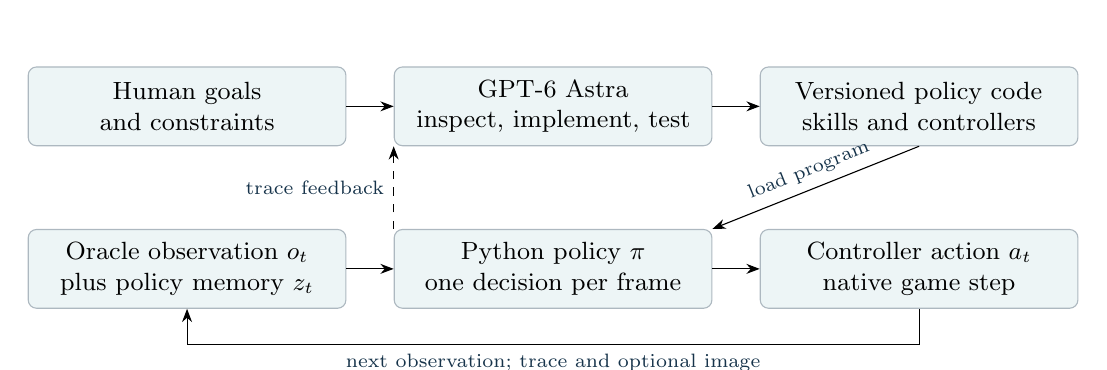
\begin{tikzpicture}[font=\small,>=Stealth,
 box/.style={draw=ink!35,rounded corners=3pt,fill=wash,align=center,minimum height=1cm,text width=3.8cm},
 lab/.style={font=\scriptsize,text=ink}]
\node[box] (human) {Human goals\\and constraints};
\node[box,right=0.6cm of human] (agent) {GPT-6 Astra\\inspect, implement, test};
\node[box,right=0.6cm of agent] (program) {Versioned policy code\\skills and controllers};
\draw[->] (human)--(agent); \draw[->] (agent)--(program);
\node[box,below=1.05cm of human] (state) {Oracle observation $o_t$\\plus policy memory $z_t$};
\node[box,below=1.05cm of agent] (policy) {Python policy $\pi$\\one decision per frame};
\node[box,below=1.05cm of program] (engine) {Controller action $a_t$\\native game step};
\draw[->] (state)--(policy); \draw[->] (policy)--(engine);
\draw[->] (program.south)--node[lab,above,sloped]{load program}(policy.north east);
\draw[->] (engine.south)--++(0,-0.45)-|node[lab,pos=.25,below]{next observation; trace and optional image}(state.south);
\draw[->,dashed] (policy.north west)--node[lab,left]{trace feedback}(agent.south west);
\end{tikzpicture}
\caption{Two timescales. The coding agent revises the program during development. The evaluated rollout executes fixed policy code; it does not query the language model for each action.}
\end{figure}

The contribution is a working integration and documented case study: an explicit oracle API, a compositional controller spanning eight stars and a boss encounter, and artifacts that connect observations to actions and verified progress. We make no claim of algorithmic novelty or superiority over alternative agents.

\clearpage
\section{Task, environment, and observation contract}
\subsection{The evaluated objective}
The episode begins on castle grounds (level 16) with all 26 saved star masks and save flags zero. ``Fresh start'' means this empty-save, post-intro starting condition: the intro cinematic is skipped, and the native adapter performs its standard 120-frame warmup before observation frame zero. Reported game times start at API frame zero. The policy must earn eight distinct saved star bits and the first Bowser key during one continuous episode.

The environment extends Gumbo64/sm64-AI, a Python interface to a native C game port derived from sm64ex-coop~\cite{gumbo}. It is not N64 emulation. Our \code{progression} mode restores dialogues, act selection, NPC interactions, ordinary deaths and exits, camera/HUD behavior, and local object updates relative to the scaffold's training shortcuts. Local area clocks advance with physics frames. Remaining differences include the skipped intro, single-player build (\code{MAX\_PLAYERS=1}), and Mario-relative stick controls. These qualifications preclude treating the result as a retail-console benchmark.

\subsection{An oracle observation is not the entire engine state}
Let $x_t$ denote the hidden native engine state and $o_t=H(x_t)$ the exported observation. The API's \code{get\_state()} returns $o_t$, a bounded, privileged view. It does not serialize all engine memory, and we do not establish that it is Markov sufficient. The policy also retains memory $z_t$, including its current skill, waypoint, and local counters.

\begin{table}[h]\centering\small
\begin{tabularx}{\linewidth}{@{}p{2.3cm}YY@{}}
\toprule
Component & Exported information & Important limitation \\
\midrule
Mario & Position, velocity, facing/angular velocity, action, health, contact and object references & Action IDs and references are privileged engine information. \\
Camera & Position, focus, field of view, roll & Approximate pose/FOV, not calibrated pixel intrinsics. \\
Geometry & Floor/wall/ceiling references and 18 sampled rays & No complete neighborhood mesh; a surface reference need not mean contact. \\
Objects & Nearest 64 within 6,000 units; IDs, behavior, position, velocity, action, timers and interaction bounds & Bounded and possibly truncated; includes off-screen information. \\
Progress/UI & Course/act, saved star masks, save flags, dialogue/menu/transition state & Save bits and hidden UI state are unavailable to a purely visual policy. \\
\bottomrule
\end{tabularx}
\caption{Observation ABI 3. Coordinates use world XYZ with Y up; velocity is in game units per physics frame. Object IDs identify episode-local allocations, not persistent semantic identities.}
\end{table}

The geometry query casts eight horizontal rays, nine downward grid rays, and one upward ray. These samples support local diagnosis, but unsampled space remains unknown. Authored navigation landmarks come separately from level source inspection; a sparse observation is not evidence that the policy discovered a complete map.

\subsection{Execution and reset semantics}
The public contract is \code{reset(level, spawn\_state)}, \code{step(action, n\_frames)}, \code{get\_state()}, \code{save\_state()/load\_state()}, and \code{render()}. Each reset owns a fresh process and save directory because the native engine has global C/Lua state. Rendering does not advance physics. Checkpoints are verified action replays with fingerprints and observation-history checks, not instantaneous native memory snapshots; restore cost grows with history length.

Curriculum probes use level resets and replay checkpoints during development. The evaluated campaign uses no custom spawn, mid-episode reset, checkpoint restore, position write, or save modification by the policy. Its interface returns only controller actions. Ordinary in-game doors, paintings, and warps remain available.

\clearpage
\section{Hierarchical code as policy}
\subsection{Skill composition and feedback}
The implemented technique is \textbf{hierarchical code-as-policy with model-based feedback control}. At runtime,
\begin{equation}
 (a_t,z_{t+1})=\pi(o_t,z_t), \qquad x_{t+1}=F(x_t,a_t),
\end{equation}
with one policy decision per physics frame. A finite-state campaign controller dispatches castle navigation and course-specific skills using level transitions and observed progress. Each skill manages its own phases and completion conditions. Shared controllers implement heading control, ordinary-jump steering, and object-centered ground pounds. Specialized code handles sliding, swimming, platform boarding, owl flight, cannon aiming, and the Bowser fight.

The hierarchy resembles temporally extended skills~\cite{options}, but its route and transitions are authored. There is no learned option policy, reward optimization, online tree search over the full game, or trained world model. Some interactions deliberately use fixed timing windows; observation feedback does not make every part of the program adaptive.

For ground steering to target $(x^*,z^*)$, let $d_x=x^*-x$, $d_z=z^*-z$, and let $\psi$ be Mario's yaw in radians. The shared controller computes
\begin{equation}
 e=\wrap_{[-\pi,\pi)}(\operatorname{atan2}(d_x,d_z)-\psi),\qquad
 (u_x,u_y)=\operatorname{round}(-M\sin e,\ M\cos e).
\end{equation}
Here $M$ is a chosen stick magnitude. This mapping depends on the fork's Mario-relative input convention; it is not portable unchanged to camera-relative controls.

During an ordinary jump, facing is locked. The controller projects target error into forward and lateral components, $d_\parallel=d_x\sin\psi+d_z\cos\psi$ and $d_\perp=d_x\cos\psi-d_z\sin\psi$, then uses a small source-informed inverse dynamics model:
\begin{align}
 v^*&=\clip(0.18d_\parallel,-12,v_{\max}),\\
 c_\parallel&=\clip((v^*-v_{\rm forward}+0.35)/1.5,-1,1),\\
 c_\perp&=\clip(0.15d_\perp/10,-1,1).
\end{align}
The implementation maps these terms through the game's stick-magnitude response and compensates for its six-unit input dead zone. It holds A for jump height. This local approximation applies to ordinary jumps; other movement modes need different skills. It is feedback control rather than model predictive control over a planned horizon.

\subsection{Two inspectable decisions}
For the Chain Chomp post, \code{GroundPoundObject} issues Z when Mario is airborne, horizontal target error is below 32 units, and his feet are more than five units above the post top. In the recorded decision from input frame 1,466 to outcome frame 1,467, the error is 28.77 units and height above the top is 46.62 units. All three predicates hold, and the final recorded action is neutral stick with Z pressed. These are logged branch conditions, not a generated explanation after the event.

For Bowser, the policy circles toward the observed tail, grabs it, and spins. It selects a bomb by angular alignment and releases with B when the absolute yaw angular velocity exceeds 3,800 engine angle units per frame and absolute aim error is below 0.15 radians. After the encounter, it approaches the observed key. The evaluator separately checks the saved key flag.

\subsection{Development procedure and agent attribution}
GPT-6 Astra served as the coding/development agent: inspecting source, implementing controllers, running probes, examining failures, and revising code. Human direction supplied goals and priorities. Replay checkpoints shortened local iteration; the final validation restarted from an empty save. The model name is session attribution, not an experimental comparison between model versions. We did not collect a complete accounting of prompts, model calls, tokens, costs, human interventions, or development trials, so none is inferred from rollout timing.

\clearpage
\section{Evaluation and observed result}
\subsection{Independent success verification}
The evaluator rejects a non-castle-grounds start, any initially collected star, or an initially present first key. Let $m_c(t)$ be course $c$'s saved star mask and $f(t)$ the save flags. Success is first recorded when
\begin{equation}
 \sum_{c=0}^{25}\popcount(m_c(t)\mathbin{\&}127)\geq8
 \quad\land\quad (f(t)\mathbin{\&}16)\ne0.
\end{equation}
This check is independent of policy phase names and the HUD star count. The final masks are 32 for Bob-omb Battlefield, 23 for Whomp's Fortress, 3 for Princess's Secret Slide, and 1 for the Secret Aquarium; other masks are zero. Final flags are 27,665, including the first-key bit 16. The evaluator leaves whole-game completion unknown.

\begin{table}[h]\centering\small
\begin{tabularx}{\linewidth}{@{}rYr r@{}}
\toprule
Order & Milestone & API frame & Game time \\
\midrule
1 & BOB: Behind Chain Chomp's Gate & 1,769 & 0:58.97 \\
2 & Princess's Secret Slide: under 21 seconds & 4,005 & 2:13.50 \\
3 & Princess's Secret Slide: box star & 5,694 & 3:09.80 \\
4 & Secret Aquarium: red coins & 9,105 & 5:03.50 \\
5 & WF: Chip Off Whomp's Block & 12,892 & 7:09.73 \\
6 & WF: To the Top of the Fortress & 16,246 & 9:01.53 \\
7 & WF: Fall onto the Caged Island & 17,218 & 9:33.93 \\
8 & WF: Shoot into the Wild Blue & 19,113 & 10:37.10 \\
-- & Enter Bowser in the Dark World & 20,380 & 11:19.33 \\
-- & Enter Bowser battle & 24,529 & 13:37.63 \\
-- & Obtain first Bowser key & 26,540 & 14:44.67 \\
\bottomrule
\end{tabularx}
\caption{Observed route, including castle travel and dialogue time. Game time is API frame divided by 30, not wall time or a speedrunning-category timer. BOB and WF abbreviate Bob-omb Battlefield and Whomp's Fortress.}
\end{table}

\begin{table}[h]\centering\small
\begin{tabularx}{\linewidth}{@{}Yrr@{}}
\toprule
Measurement & Initial success & Instrumented rerun \\
\midrule
Run suffix & \code{attempt-03} & \code{debug-01} \\
Success frame / unique stars & 26,540 / 8 & 26,540 / 8 \\
Deaths / minimum health & 0 / 5 of 8 & 0 / 5 of 8 \\
Recorded decisions / images & 26,600 / 8,868 & 26,600 / 8,868 \\
Episode wall time (s) & 142.05 & 140.44 \\
Policy loop wall time (s) & 141.53 & 139.86 \\
Physics frames per loop second & 187.94 & 190.20 \\
\bottomrule
\end{tabularx}
\caption{Single-session native runs on Apple Silicon macOS 26.5.2, Python 3.14.4. Oracle mode, one-frame decisions, 480$\times$270 images every three frames; a 60-frame tail follows success. Timing is descriptive and includes recording overhead.}
\end{table}

The instrumented fresh-save rerun reproduces the initial observation and every recorded action and resulting observation in the successful run. Diagnostics intentionally differ. This supports noninterference of the added logging on this trajectory. It does not establish hidden-state equality, robustness to perturbations, or a general native determinism guarantee. Earlier development attempts used changing implementations and are not independent trials of a frozen policy. We therefore report neither a success percentage nor a confidence interval. Two isolated course-and-fight probes provide additional development evidence but are not counted as full campaigns.

\clearpage
\section{Making the policy observable}
\subsection{A synchronized game and state debugger}
The dashboard pairs recorded game images with an interactive 3D rendering of the exported observation. Mario is a capsule proxy with facing and velocity arrows; objects have behavior-colored proxies and optional interaction bounds. Contact references and ray-hit triangles expose observed collision geometry. Camera pose, target markers, authored waypoints, a recent trajectory, and a preceding-state ghost make motion and intent visible. Orbit, follow, top-down, and approximate game-camera views support inspection.

The display is intentionally explicit about measurement limits. The grid is a ruler, not reconstructed terrain. Object hitboxes are not collision meshes. Ray misses do not establish free space outside the sampled rays. Objects omitted from a truncated query are not assumed destroyed. Images have their own frame labels because recording is sparse. A complete oracle reconstruction of the scene is neither available nor claimed.

\subsection{Preserving the direction of causality}
A trace row records $(a_t,o_{t+1})$. Its input is $o_t$, taken from the preceding row or the initial observation. The debugger presents
\[
 \boxed{\text{input observation}}\ \longrightarrow\
 \boxed{\text{evaluated controls and gates}}\ \longrightarrow\
 \boxed{\text{final action}}\ \longrightarrow\
 \boxed{\text{observed outcome}}.
\]
Instrumented helpers record actual targets, errors, intermediate controls, and branch predicates during execution. Later overrides are distinguished from earlier intermediate outputs. The viewer does not rerun current policy code to explain old recordings. A direct action without recorded conditions remains unexplained beyond the available trace. This is an execution log, not access to a language model's private reasoning.

This distinction also matters for future training data: using a row's resulting observation as the input for its own action would leak future information. State, action duration, and image timestamps must remain aligned. The dashboard serves small indexed state pages and caches a bounded number of pages, avoiding a full multi-gigabyte oracle trace in browser memory.

\subsection{A concrete development failure}
The Bowser course's rotating platforms required more than a target coordinate. Boarding too early led to collision with the next platform overhead. The revised skill waits until the target platform is descending and crosses an authored X-position threshold before approaching. This example illustrates the useful unit of revision: a condition inside a reusable skill, tied to an observed failure. It does not establish robustness across arbitrary platform phases or routes.

\section{Systems design and performance scope}
The native fast path omits GPU submission and pixel readback on frames that need no image. CPU scene traversal and animation callbacks remain because removing them can change gameplay. The process-isolated Python API is implemented with the standard library; native C performs physics and gameplay. Independent episodes can run in parallel, each with its own save directory. The demonstrated campaign is one continuous, single-worker episode.

A separate earlier benchmark measured 4,331.9 versus 14,284.3 aggregate physics frames/s, a 3.30$\times$ increase, across 12 basic-observation episodes with four concurrent workers. It used 1,800 decisions of four frames each, 128$\times$72 endpoint images, and no-op, random, and exploration policies. All 21,600 action/observation pairs and initial observations matched. These are single sequential suite measurements on the development machine. They use different binaries, observations, and capture density from the campaign and cannot be substituted for its approximately 188--190 recorded frames/s. Those baseline policies collected no stars; throughput alone is not gameplay competence.

\clearpage
\section{Related work}
\textbf{Language models writing control programs.} Liang et al.'s \emph{Code as Policies} formalizes language-model-generated programs that compose perception outputs, geometric calculations, and control APIs~\cite{cap}. Our use of executable feedback code follows that general direction. Here the work is a source-informed game-controller case study with substantial iterative engineering, rather than a replication of their robotic instruction-generalization evaluation.

\textbf{Executable skills in games.} Voyager combines an automatic curriculum, a growing code skill library, and execution feedback in Minecraft~\cite{voyager}. It is a close precedent for treating programs as reusable agent skills. Our campaign instead has a fixed human-directed objective and an authored route; it does not demonstrate autonomous open-ended skill discovery or transfer to unseen worlds.

\textbf{Programmatic policies and hierarchy.} Programmatically Interpretable Reinforcement Learning searches for symbolic policies using a neural policy as guidance~\cite{pirl}. We share the inspectable program representation but do not use its neural training or program-search algorithm. The options framework provides the classical account of temporally extended closed-loop behavior~\cite{options}; our explicit skills use that broad organizational idea without learning option selection or termination.

\textbf{Code generation around RL.} Eureka uses coding language models to generate and improve reward functions, then acquires behavior through reinforcement learning~\cite{eureka}. Here generated code directly specifies the action policy. RL could later replace selected controllers, but the present milestone contains no RL training. Gumbo64/sm64-AI supplies the native interface foundation and includes curiosity-learning experiments~\cite{gumbo}; we do not claim to have originated that engine interface or compare task success against those experiments.

These connections locate the project in an established line of work. Different environments, observation privileges, development budgets, and evaluation protocols rule out numerical performance rankings from this case study.

\section{Limitations and next experiments}
\textbf{Scope and robustness.} The result covers a specific eight-star route and first key, not all of Super Mario 64. Source-informed landmarks, object behavior IDs, save bits, and exact state remove difficult perception and discovery problems. Identical reruns provide limited evidence about recovery from altered momentum, timing, observation noise, or missed inputs. A next evaluation should freeze the implementation and report success, failures, deaths, and completion time across a preregistered set of such perturbations, with separately labeled curriculum starts and full campaigns.

\textbf{Scalability is an interface property, not a demonstrated outcome.} Shared controllers and skill boundaries allow local replacements and regression tests. They do not guarantee that the effort needed for each new star stays small. Useful comparisons include waypoint-only control versus feedback, feedback with different observation subsets, and authored skills versus learned replacements under the same start states and budget. The current record does not support claims about sample efficiency or superiority to RL.

\textbf{From oracle to estimated state.} A planned second stage replaces oracle inputs with a recurrent estimator,
\begin{equation}
 b_t=f_\phi(b_{t-1},a_{t-1},\Delta t_{t-1},I_t),\qquad
 \hat{o}_t=g_\phi(b_t),\qquad (a_t,z_{t+1})=\pi(\hat{o}_t,z_t).
\end{equation}
Here $I_t$ is the current image and $b_t$ summarizes earlier images, actions, and estimated state. This is proposed future work. Oracle traces can supply supervision during training, but inference must use the estimator's own history; hidden save bits and object timers cannot be silently retained as policy inputs. Some fields will need uncertainty or alternative abstractions rather than exact reconstruction. Evaluation should measure downstream task success as well as state error, while keeping the external success verifier privileged and independent.

\clearpage
\section{Reproducibility and evidence}
The local artifacts are \code{artifacts/first-bowser-attempt-03/} and \code{artifacts/first-bowser-debug-01/}, each with \code{session-000/}. Session files include configuration, JSONL actions/observations, rollout metadata, result metrics, logs, and recorded images. The instrumented run additionally has \code{debug-validation.json}. Full file identities and claim-to-source mappings accompany this report in \code{docs/publication/evidence.md}.

To run the campaign from the repository root after supplying a compatible ROM and building the native library:
\begin{quote}\small\ttfamily
make build\\
PYTHONPATH=src python3 -m sm64\_policy benchmark \textbackslash\\
\hspace*{1em}--policies first-bowser --seeds 0 --workers 1 \textbackslash\\
\hspace*{1em}--gameplay-mode progression --level 16 \textbackslash\\
\hspace*{1em}--steps 36000 --frame-skip 1 --timeout 1800 \textbackslash\\
\hspace*{1em}--record-every 3 --width 480 --height 270 \textbackslash\\
\hspace*{1em}--output artifacts/paper-reproduction-NEW\\
make dashboard
\end{quote}
Use a new output directory. Verify \code{task.success} and \code{termination=task\_success}, not just process status. Recorded local playback is available through the dashboard; local addresses are not public data-release URLs. ROMs, extracted assets, binaries, saves, and run artifacts are excluded from Git.

\textbf{Provenance caveats.} The recorded Git identifier is an upstream/base revision with local changes, not a complete frozen release of this implementation. The manifest's source hash and binary hash add evidence, but a source hash alone does not provide an archived checkout. The campaign manifests also retain a stale BOB/scaffold \code{scope} string; per-session configuration, native traces, and results identify the actual progression-mode campaign. Historical artifacts are preserved rather than silently rewritten. A public release should include a reviewed source revision and portable artifact index. Timing metadata identifies Apple Silicon/macOS and Python versions but does not record the exact chip model or controlled machine load.

\textbf{Conclusion.} Under the specified oracle and native-port conditions, a program developed by GPT-6 Astra with human direction completes the fresh-save eight-star and first-Bowser-key objective. The useful result is both the behavior and its inspectable representation: skills, measured conditions, controller actions, and independently verified progress. Broader reliability and vision-based control remain experiments to perform.

\begin{thebibliography}{9}\small
\bibitem{cap} J. Liang, W. Huang, F. Xia, P. Xu, K. Hausman, B. Ichter, P. Florence, and A. Zeng. \emph{Code as Policies: Language Model Programs for Embodied Control}. 2022. \href{https://arxiv.org/abs/2209.07753}{arXiv:2209.07753}.
\bibitem{voyager} G. Wang, Y. Xie, Y. Jiang, A. Mandlekar, C. Xiao, Y. Zhu, L. Fan, and A. Anandkumar. \emph{Voyager: An Open-Ended Embodied Agent with Large Language Models}. 2023. \href{https://arxiv.org/abs/2305.16291}{arXiv:2305.16291}.
\bibitem{pirl} A. Verma, V. Murali, R. Singh, P. Kohli, and S. Chaudhuri. \emph{Programmatically Interpretable Reinforcement Learning}. ICML, PMLR 80:5045--5054, 2018. \href{https://proceedings.mlr.press/v80/verma18a.html}{Proceedings}.
\bibitem{options} R. S. Sutton, D. Precup, and S. Singh. \emph{Between MDPs and Semi-MDPs: A Framework for Temporal Abstraction in Reinforcement Learning}. Artificial Intelligence 112(1--2):181--211, 1999. \href{https://people.cs.umass.edu/~barto/courses/cs687/Sutton-Precup-Singh-AIJ99.pdf}{Author paper}.
\bibitem{eureka} Y. J. Ma, W. Liang, G. Wang, D.-A. Huang, O. Bastani, D. Jayaraman, Y. Zhu, L. Fan, and A. Anandkumar. \emph{Eureka: Human-Level Reward Design via Coding Large Language Models}. 2023. \href{https://arxiv.org/abs/2310.12931}{arXiv:2310.12931}.
\bibitem{gumbo} Gumbo64 and upstream contributors. \emph{sm64-AI}. Native Super Mario 64/Python interface, derived from sm64ex-coop. \href{https://github.com/Gumbo64/sm64-AI}{GitHub repository}. Accessed September 28, 2026.
\end{thebibliography}
\end{document}
